\documentclass[11pt]{article}

\usepackage[a4paper,margin=1in]{geometry}
\usepackage[T1]{fontenc}
\usepackage{microtype}
\usepackage{amsmath,amssymb}
\usepackage{booktabs}
\usepackage{graphicx}
\usepackage{float}
\usepackage{hyperref}

\setlength{\parindent}{0pt}
\setlength{\parskip}{0.45em}

\title{\textbf{Exercise 1 -- Introduction to Speech Recognition}}
\author{Gal Noy (209346485) \\ Amit Ezer (316097575)}
\date{}

\begin{document}
\maketitle
\vspace{-1.5em}

\section{Question 1 -- DFT and Windowing}

\subsection*{(a)--(b) DFT of the First Signal}

The signal contains $N=400$ samples at $f_s=16{,}000$ Hz, giving a duration of $25$ ms and a frequency resolution of $\Delta f=f_s/N=40$ Hz. We construct it as
\[
 s_1[n]=\sum_{i=1}^{3} A_i\cos\!\left(2\pi f_i\frac{n}{f_s}+\phi_i\right),
 \qquad 0\le n<N.
\]
The DFT is computed by multiplying the signal by the explicitly constructed matrix
\[
 W_{k,n}=e^{-j2\pi kn/N},\qquad \mathbf{X}_1=W\mathbf{s}_1.
\]
Only bins $k=0,\ldots,199$ are displayed: for a real signal, $X[N-k]=\overline{X[k]}$, so the negative-frequency half is redundant (the Nyquist bin $k=200$ is a separate boundary bin). All spectra use $20\log_{10}(|X[k]|/P)$, where $P$ is the maximum coefficient magnitude of the original signal. Values below $-80$ dB are clipped for display; each window comparison uses the same $P$ for both curves.

\begin{figure}[H]
\centering
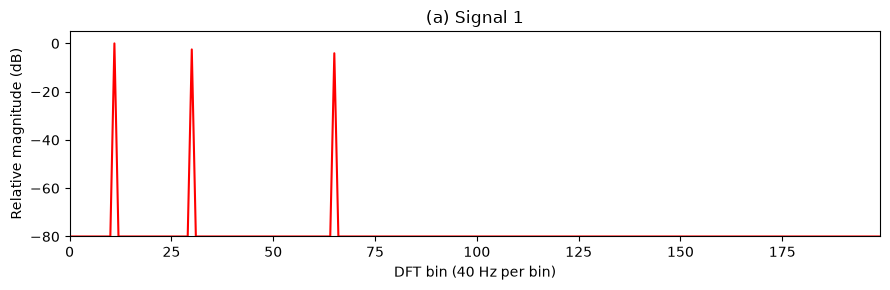
\includegraphics[width=0.92\linewidth]{figures/signal_1_dft.png}
\caption{DFT magnitude of the first signal (relative dB).}
\end{figure}

\subsection*{(c) Amplitudes and Phases of the First Signal}

For a tone aligned with bin $k=f/\Delta f$, its amplitude and phase are $A=2|X[k]|/N$ and $\phi=\arg X[k]$. All three frequencies are bin-aligned, yielding:

\begin{center}
\begin{tabular}{rrrr}
\toprule
Tone (Hz) & Bin $k$ & Amplitude & Phase (rad) \\
\midrule
440  & 11 & 0.40000 &  0.78540 \\
1200 & 30 & 0.30000 &  0.00000 \\
2600 & 65 & 0.25000 & -2.35619 \\
\bottomrule
\end{tabular}
\end{center}

\subsection*{(d)--(e) DFT, Amplitudes and Phases of the Second Signal}

The new frequencies are $450$, $1100$, and $2550$ Hz. Their DFT-bin positions are $11.25$, $27.5$, and $63.75$, respectively. None is bin-aligned, so \textbf{spectral leakage} spreads the energy over neighboring bins instead of producing isolated peaks.

\begin{figure}[H]
\centering
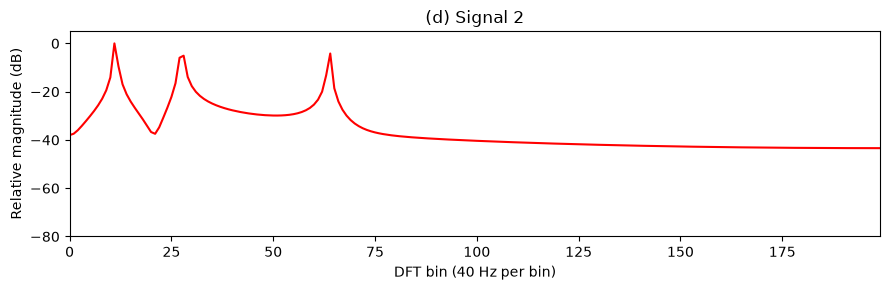
\includegraphics[width=0.92\linewidth]{figures/signal_2_dft.png}
\caption{DFT magnitude of the second signal, showing spectral leakage (relative dB).}
\end{figure}

Using the closest bins (both equally close bins for 1100 Hz) gives:

\begin{center}
\begin{tabular}{rrrr}
\toprule
Tone (Hz) & Bin $k$ & Amplitude & Phase (rad) \\
\midrule
450  & 11 & 0.35950 &  1.55805 \\
1100 & 27 & 0.18144 &  1.54371 \\
1100 & 28 & 0.20022 & -1.54607 \\
2550 & 64 & 0.22197 & -3.11427 \\
\bottomrule
\end{tabular}
\end{center}

The selected bins correspond to $440$, $1080$, $1120$, and $2560$ Hz, respectively. These are amplitudes and phases of the DFT coefficients at those bin frequencies, not exact recovery of the original tone parameters.

\subsection*{(f) Hamming Window}

Both signals are multiplied by the $N$-sample Hamming window
\[
 w[n]=\frac{25}{54}-\frac{21}{54}\cos\!\left(\frac{2\pi n}{N}\right),
 \qquad 0\le n<N.
\]
For the first signal, all tones are bin-aligned, so the original DFT has no spectral leakage. Windowing lowers the peaks and spreads energy into adjacent bins. For the second signal, which already has leakage, the window reduces the distant sidelobes but widens and lowers the main peaks.

\begin{figure}[H]
\centering
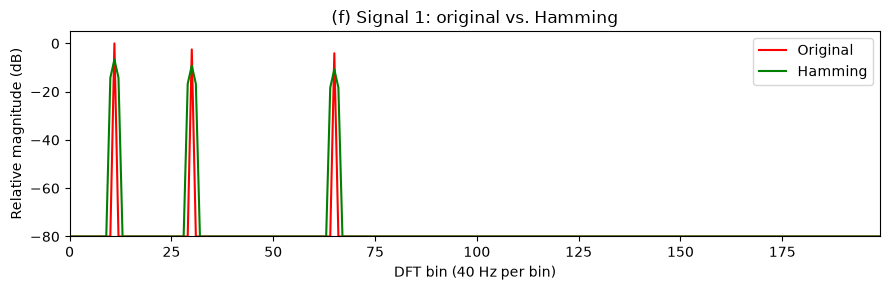
\includegraphics[width=0.86\linewidth]{figures/signal_1_hamming.png}
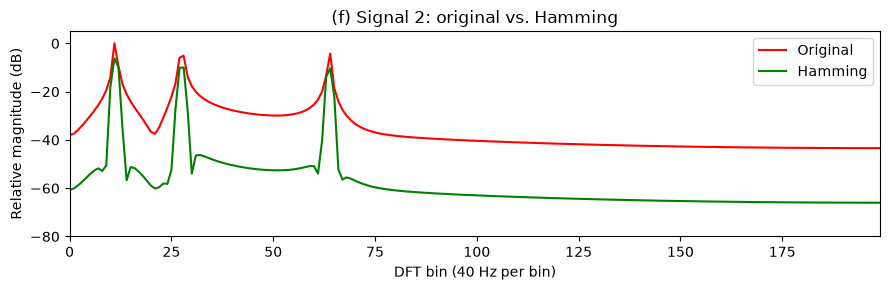
\includegraphics[width=0.86\linewidth]{figures/signal_2_hamming.png}
\caption{Original DFT (red) and windowed DFT (green) for each signal.}
\end{figure}

\subsection*{(g) Amplitudes and Phases after Windowing}

The same coefficient-based estimates, now obtained from the windowed DFTs, are:

\begin{center}
\begin{tabular}{llrrr}
\toprule
Signal & Tone (Hz) & Bin $k$ & Amplitude & Phase (rad) \\
\midrule
$ s_1 w$ & 440  & 11 & 0.18519 &  0.78540 \\
         & 1200 & 30 & 0.13889 &  0.00000 \\
         & 2600 & 65 & 0.11574 & -2.35619 \\
\midrule
$ s_2 w$ & 450  & 11 & 0.17601 &  1.56887 \\
         & 1100 & 27 & 0.11248 &  1.56756 \\
         & 1100 & 28 & 0.11385 & -1.56758 \\
         & 2550 & 64 & 0.10980 & -3.13751 \\
\bottomrule
\end{tabular}
\end{center}

For the first signal, the phases remain unchanged and the peak amplitudes are reduced by the average window weight, $\frac{1}{N}\sum_n w[n]=25/54\approx0.463$. For the second signal, the window changes the distribution of energy between bins, affecting both the coefficient-based amplitudes and phases. The reported values refer to the same selected bin frequencies as in part (e).

\clearpage
\section{Question 2 -- Multivariate Gaussian Models}

For $M$ equally weighted vectors $\mathbf{x}_i\in\mathbb{R}^d$, we estimate
\[
\boldsymbol\mu=\frac{1}{M}\sum_{i=1}^{M}\mathbf{x}_i,
\qquad
\Sigma=\frac{1}{M}\sum_{i=1}^{M}(\mathbf{x}_i-\boldsymbol\mu)(\mathbf{x}_i-\boldsymbol\mu)^T.
\]
The diagonal model retains only the diagonal of $\Sigma$. For both models, with normalization constant $C=(2\pi)^{-d/2}|\Sigma|^{-1/2}$,
\[
\log p(\mathbf{x})=\log C-\frac{1}{2}(\mathbf{x}-\boldsymbol\mu)^T
\Sigma^{-1}(\mathbf{x}-\boldsymbol\mu).
\]
The inverse covariance and $\log C$ are computed once during initialization.

\subsection*{(a) Models Estimated from \texttt{data\_1.csv}}

Both models have mean $\boldsymbol\mu_1=(-0.098231,\,-0.097654,\,0.084253)^T$.
The diagonal covariance is represented by the variance vector
\[
\boldsymbol\sigma_1^2=(11.300731,\ 1.480702,\ 6.454034),
\]
while the full covariance is
\[
\Sigma_1=\begin{pmatrix}
11.300731 & -0.032292 & 0.258590\\
-0.032292 & 1.480702 & -0.079734\\
0.258590 & -0.079734 & 6.454034
\end{pmatrix}.
\]
The normalization constants are $C_{1,\mathrm{diag}}=0.006109807$ and $C_{1,\mathrm{full}}=0.006114799$.

\subsection*{(b) Log-Likelihoods for \texttt{query\_1.csv}}

\begin{center}
\begin{tabular}{rrr}
\toprule
Query & Diagonal & Full \\
\midrule
1  & -9.598437 & -9.595777 \\
2  & -6.439222 & -6.397500 \\
3  & -7.255353 & -7.226701 \\
4  & -6.604090 & -6.562551 \\
5  & -5.701920 & -5.692899 \\
6  & -5.308776 & -5.309611 \\
7  & -7.417854 & -7.458339 \\
8  & -7.273178 & -7.289781 \\
9  & -5.601006 & -5.583757 \\
10 & -7.302052 & -7.275010 \\
\bottomrule
\end{tabular}
\end{center}

\subsection*{(c) Models Estimated from \texttt{data\_2.csv}}

Both models have mean $\boldsymbol\mu_2=(5.298580,\,-0.881825,\,1.290526)^T$.
The diagonal covariance is represented by
\[
\boldsymbol\sigma_2^2=(8.886413,\ 6.460199,\ 3.886459),
\]
and the full covariance is
\[
\Sigma_2=\begin{pmatrix}
8.886413 & 3.424745 & 1.619543\\
3.424745 & 6.460199 & -1.892735\\
1.619543 & -1.892735 & 3.886459
\end{pmatrix}.
\]
The normalization constants are $C_{2,\mathrm{diag}}=0.004250764$ and $C_{2,\mathrm{full}}=0.006116646$.

\subsection*{(d) Log-Likelihoods for \texttt{query\_2.csv}}

\begin{center}
\begin{tabular}{rrr}
\toprule
Query & Diagonal & Full \\
\midrule
1  & -8.336550 & -9.595454 \\
2  & -6.975472 & -6.397200 \\
3  & -8.348692 & -7.226405 \\
4  & -7.369369 & -6.562250 \\
5  & -5.631708 & -5.692596 \\
6  & -5.646387 & -5.309307 \\
7  & -8.762895 & -7.458044 \\
8  & -7.700626 & -7.289480 \\
9  & -5.904931 & -5.583454 \\
10 & -6.289201 & -7.274711 \\
\bottomrule
\end{tabular}
\end{center}

\subsection*{(e) Explanation of the Differences}

In the first dataset, the off-diagonal entries of $\Sigma_1$ are small relative to the variances, so the diagonal and full models give similar log-likelihoods. In the second dataset, the off-diagonal entries of $\Sigma_2$ are substantial. Ignoring these dependencies changes the diagonal-model scores considerably.

The two full models have nearly equal normalization constants, and the quadratic terms in the log-likelihood formula are also nearly equal for corresponding queries. Consequently, their log-likelihoods in (b) and (d) differ by at most $0.000324$.

\end{document}
